\subsection{Trigonometric Functions}
There are six basic trigonometric functions:
\begin{multicols}{2}
\begin{itemize}
	\item Sine (abbreviated by $\sin$)
	\item Cosine (abbreviated by $\cos$)
	\item Tangent (abbreviated by $\tan$)
	\item Cosecant (abbreviated by $\csc$)
	\item Secant (abbreviated by $\sec$)
	\item Cotangent (abbreviated by $\cot$)
\end{itemize}
\end{multicols}

We first describe trigonometric functions in terms of ratios of two sides of a \ifont{right angle triangle} containing the angle $\theta$. 

$$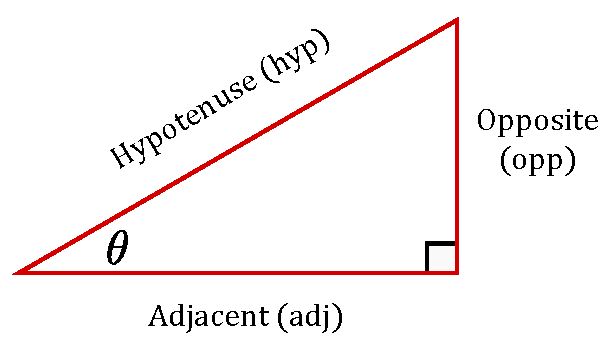
\includegraphics[width=2.5in]{images/trig2}$$

With reference to the above triangle, for an acute angle $\theta$ (that is, $0\leq\theta<\pi/2$), the six trigonometric functions can be described as follows:
$$\begin{array}{ccc}
\ds\sin\theta=\frac{\rm opp}{\rm hyp}&\qquad&\ds\csc\theta=\frac{\rm hyp}{\rm opp}\\
\\
\ds\cos\theta=\frac{\rm adj}{\rm hyp}&\qquad&\ds\sec\theta=\frac{\rm hyp}{\rm adj}\\
\\
\ds\tan\theta=\frac{\rm opp}{\rm adj}&\qquad&\ds\cot\theta=\frac{\rm adj}{\rm opp}\\
\end{array}$$

\begin{formulabox}[Mnemonic]
The mnemonic \ifont{SOH CAH TOA} is useful in remembering how trigonometric functions of acute angles relate to the sides of a right triangle.
\end{formulabox}

This description does not apply to \ifont{obtuse} or \ifont{negative angles}.
To define the six basic trigonometric functions we first define sine and cosine as the lengths of various line segments from a unit circle, and then we define the remaining four basic trigonometric functions in terms of sine and cosine.

Take a line originating at the origin (making an angle of $\theta$ with the positive half of the $x$-axis) and suppose this line intersects the unit circle at the point $(x,y)$.
The $x$- and $y$-coordinates of this point of intersection are equal to $\cos\theta$ and $\sin\theta$, respectively.
$$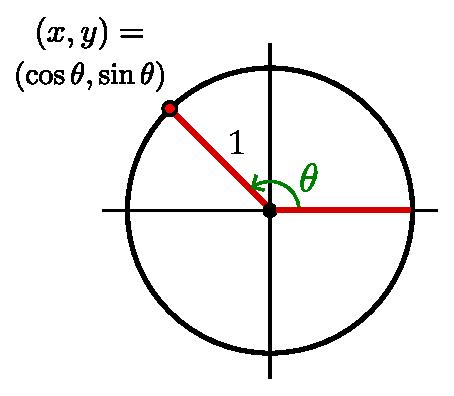
\includegraphics[width=2.3in]{images/trig3}$$
For angles greater than $2\pi$ or less than $-2\pi$, simply continue to rotate around the circle.
In this way, sine and cosine become periodic functions with period $2\pi$:
$$\sin\theta = \sin\left(\theta + 2\pi k \right)\qquad\qquad \cos\theta = \cos\left(\theta + 2\pi k \right)$$
for any angle $\theta$ and any integer $k$.

Above, only sine and cosine were defined directly by the circle.
We now define the remaining four basic trigonometric functions in terms of the functions $\sin\theta$ and $\cos\theta$:
$$\tan\theta = \frac{\sin\theta}{\cos\theta} \qquad \sec\theta = \frac{1}{\cos\theta} \qquad \csc\theta = \frac{1}{\sin\theta} \qquad \cot\theta = \frac{\cos\theta}{\sin\theta}$$